\section{Proposed Approach}
\subsection{Large Margin Cotangent Loss (LMCot)}
Large Margin Loss is generally very common in learning similarity, Ex: SphereFace \cite{liu2017sphereface}, SV-AM-Softmax \cite{wang2018support}, CosFace \cite{wang2018cosface}, ArcFace \cite{deng2019arcface}, AdaCos \cite{zhang2019adacos}, etc. The most common function in both competitions and applications is ArcFace, as they are effective and easy to implement.

ElasticFace-Arc \cite{boutros2022elasticface} is a method inherited from ArcFace \cite{deng2019arcface}. The main idea is to use random margin values drawn from a normal distribution in each training iteration. This method advanced state-of-the-art on seven mainstream face recognition benchmarks. Therefore, we also investigate the effects of using cosine and cotangent by implementing cotangent loss on top of ArcFace. We examine the ArcFace loss function:
\begin{equation}
\label{equation06}
    L=-\frac{1}{N}\sum\limits_{i=1}^{N}{\log }\frac{{{e}^{s\left( \cos \left( {{\theta }_{yi}}+m \right) \right)}}}{{{e}^{s\left( \cos \left( {{\theta }_{yi}}+m \right) \right)}}+\sum\limits_{j=1,j\ne {{y}_{i}}}^{n}{{{e}^{s\cos {{\theta }_{ji}}}}}},
\end{equation}
where ${{\theta }_{ji}}$ is the angle between the weight ${{W}_{j}}^{T}$ and the feature ${{x}_{i}}$. The label of ${{i}^{th}}$ is $y$, ${{\theta }_{yi}}$ is the angle between the feature ${{x}_{i}}$ and the feature of class $y$ stored in weight $W$. The margin $m$ is the penalty, and $s$ is a scale parameter.

The problem with ArcFace is that the cosine function only provides value within  $\left[ -1,1 \right]$. Hence, it is not fully representing the degrees between the angles as much as the cotangent, where the value obtained within $\left( -\infty ,+\infty  \right)$. For instance, by $j\ne y$ with small ${{\theta }_{ij}}$ and smaller ${{\theta }_{iy}}$, the cosine function will not be large enough. When the initialized weights are bad, the ${{\theta }_{iy}}$ is closer to $\pi $. As a result, the cotangent function will receive a larger loss to make the model optimize faster. This is more satisfactory for tasks that need high top-1 accuracy. LMCot is presented as follows:
\begin{equation}
\label{equation07}
    L=-\frac{1}{N}\sum\limits_{i=1}^{N}{\log }\frac{{{e}^{s\left( \cot \left( {{\theta }_{yi}}+m \right) \right)}}}{{{e}^{s\left( \cot \left( {{\theta }_{yi}}+m \right) \right)}}+\sum\limits_{j=1,j\ne {{y}_{i}}}^{n}{{{e}^{s\cot {{\theta }_{ji}}}}}}.
\end{equation}

\begin{figure*}
    \centering
    \includesvg[inkscapelatex=false, width=\textwidth]{images/LMCot_Flow.svg}
    \caption{DCNN model trained by Large Margin Cotangent Loss based on ArcFace \cite{deng2019arcface}. The $cos \left( \theta_j \right)$ (logit) for each class is obtained from the normalization of the feature $x_i$ and weight $W$, presented as $W_{j}^{T}x_{i}$. The angle between the feature $x_i$ and the weight $W$ is computed by $arccos \left( \theta_{yi} \right)$. After calculating $cot \left( \theta_{yi} + m \right)$, all logits are multiplied by the scale $s$ to go through the softmax and the cross-entropy loss. }
    \label{fig:my_label}
\end{figure*}

In bad weight initialization scenario, the cotangent function will perform better since $\cot \left( {{\theta }_{ij}} \right)$ will be very large. Other variables remain the same as those in ArcFace, we only replace the cosine function with the cotangent function. Furthermore, when the angle is enough (not too large and not too small), the cosine and cotangent functions would start getting closer to each other.


\begin{figure}
\centering
        \subfloat[Figure created by Geogebra \cite{hohenwarter2002geogebra} \label{subfig02}]{
        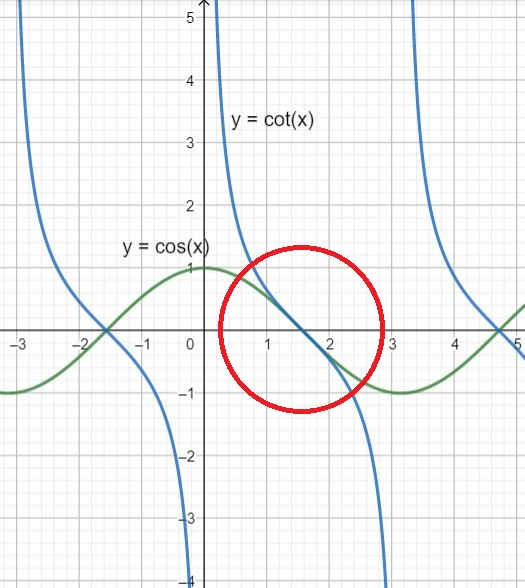
\includegraphics[width=0.48\linewidth]{images/cos-cot.JPG}}
        
    \caption{The graph represents the function $y=\cos \left( x \right)$ and the function $y=\cot \left( x \right)$ respectively. In the area of the red circle, $\cos \left( x \right)$ are close to $\cot \left( x \right)$. By convention, the angle of the two feature vectors $x\in \left[ 0,\pi  \right)$.}
    \label{figure02}

\end{figure}

Pseudo-code of LMCot in Siamese Network with backbone $B$, weight $W$, and $\varepsilon$ is the smallest value that can become the denominator.\\
\noindent\rule{\linewidth}{0.4pt}
{\raggedright \textbf{Input}: data $x$, scale $s$, margin $m$, epsilon $\varepsilon $, class number $n$, Ground-Truth ID $gt$. \par}
\noindent\rule{\linewidth}{0.4pt}
\begin{enumerate}
\item $f=\left\| B\left( x \right) \right\|$
\item $W=\left\| W \right\|$
\item $\cos \_theta=Wf$
\item $theta=\arccos \left( \cos \_theta \right)$
\item $\cot \_t=\cos \_theta /\max \left( \sin \left( theta \right),\varepsilon  \right)$
\item $\cot \_t\_m=\cos \left( theta + m \right)/\max \left(\sin \left( theta+m \right), \varepsilon \right)$
\item $one\_hot=onehot\left( gt \right)$
\item $\text{logit}=one\_hot*\cot \_t\_m + \left( 1-one\_hot \right)*\cot \_t $
\item $\text{logit}=s*\text{logit}$
\end{enumerate}
\noindent\rule{\linewidth}{0.4pt}
\leftline{\textbf{Output}: Class-wise affinity score $\text{logit}$}
\noindent\rule{\linewidth}{0.4pt}
{\raggedright In the circumstance that the arc-cosine computation becomes complicated, we can use the following pseudo-code to skip the theta computing step. \par}
\noindent\rule{\linewidth}{0.4pt}
{\raggedright\textbf{Input}: data $x$, scale $s$, margin $m$, epsilon $\varepsilon $, class number $n$, Ground-Truth ID $gt$.\par}
\noindent\rule{\linewidth}{0.4pt}
\begin{enumerate}
\item $f=\left\| B\left( x \right) \right\|$
\item $W=\left\| W \right\|$
\item $\cos \_theta=Wf$
\item $\sin \_theta=\sqrt{1-\cos \_thet{{a}^{2}}}$
\item $\cot \_theta=\cos \_theta/\max \left(\sin \_theta, \varepsilon \right)$
\item $\cos \_theta\_m=\cos \_theta*\cos \left( m \right) -\sin \_theta*\sin \left( m \right) $
\item $\sin \_theta\_m=\sin \_theta*\cos \left( m \right)+\cos \_theta*\sin \left( m \right) $ 
\item	$\cot \_theta\_m=\cos \_theta\_m/ \max \left(\sin \_theta\_m, \varepsilon \right)$
\item $one\_hot=onehot\left( gt \right)$
\item $\text{logit}=one\_hot*\cot \_theta\_m + \left( 1-one\_hot \right)*\cot \_theta $
\item $\text{logit}=s*\text{logit}$
\end{enumerate}
\noindent\rule{\linewidth}{0.4pt}
\leftline{\textbf{Output}: Class-wise affinity score $\text{logit}$}
\noindent\rule{\linewidth}{0.4pt}

\subsection{Ensemble methods}
We present the idea of integrating SphereFace \cite{liu2017sphereface}, CosFace \cite{wang2018cosface}, ArcFace \cite{deng2019arcface}, ElasticFace \cite{boutros2022elasticface} methods and use cotangent instead of cosine. 

\begin{equation}
\label{eq:ensemble}
\begin{split}
    L&=-\frac{1}{N}\sum\limits_{i=1}^{N}{\log }\frac{{{e}^{s\left( \cot \left( E\left( {{m}_{1}},{{\sigma }_{1}} \right){{\theta }_{yi}}+E\left( {{m}_{2}},{{\sigma }_{2}} \right) \right)+E\left( {{m}_{3}},{{\sigma }_{3}} \right) \right)}}}{{{e}^{s\left( \cot \left( E\left( {{m}_{1}},{{\sigma }_{1}} \right){{\theta }_{yi}}+E\left( {{m}_{2}},{{\sigma }_{2}} \right) \right)+E\left( {{m}_{3}},{{\sigma }_{3}} \right) \right)}}+I}, \\ \quad
    I&=\sum\limits_{j=1,j\ne {{y}_{i}}}^{n}{{{e}^{s\cot {{\theta }_{ji}}}}},
\end{split}
\end{equation}
where $E\left( \overline{x},\sigma  \right)$ is the normal function that returns a random value from a Gaussian distribution with the mean $\overline{x}$ and the standard deviation $\sigma $.

In addition, we present the method of combining cotangent and cosine functions.
\begin{equation}
    \begin{split}
        &L=\alpha {{L}_{\cot }}+\beta {{L}_{\cos }}, \\ \quad
        &{{L}_{\cot }} =-\frac{1}{N}\sum\limits_{i=1}^{N}{\log }\frac{{{e}^{s\left( \cot \left( E\left( {{m}_{1}},{{\sigma }_{1}} \right){{\theta }_{yi}}+E\left( {{m}_{2}},{{\sigma }_{2}} \right) \right)+E\left( {{m}_{3}},{{\sigma }_{3}} \right) \right)}}}{{{e}^{s\left( \cot \left( E\left( {{m}_{1}},{{\sigma }_{1}} \right){{\theta }_{yi}}+E\left( {{m}_{2}},{{\sigma }_{2}} \right) \right)+E\left( {{m}_{3}},{{\sigma }_{3}} \right) \right)}}+I}, \\ \quad
        &{{L}_{\cos }} =-\frac{1}{N}\sum\limits_{i=1}^{N}{\log }\frac{{{e}^{s\left( \cos \left( E\left( {{m}_{1}},{{\sigma }_{1}} \right){{\theta }_{yi}}+E\left( {{m}_{2}},{{\sigma }_{2}} \right) \right)+E\left( {{m}_{3}},{{\sigma }_{3}} \right) \right)}}}{{{e}^{s\left( \cos \left( E\left( {{m}_{1}},{{\sigma }_{1}} \right){{\theta }_{yi}}+E\left( {{m}_{2}},{{\sigma }_{2}} \right) \right)+E\left( {{m}_{3}},{{\sigma }_{3}} \right) \right)}}+I}, \\ \quad
        &\text{and } I =\sum\limits_{j=1,j\ne {{y}_{i}}}^{n}{{{e}^{s\cot {{\theta }_{ji}}}}}.
    \end{split}
\end{equation}

Finally, we divide the training process into several stages. In each stage, we use a different loss function.
